\section{Analog HCAL}
Most recent update: 2018-08-23\\
Contact person: Felix Sefkow (email: felix.sefkow@desy.de)
\subsection{Introduction}
With the advent of silicon photo-multipliers (SiPMs), the scintillator tile technology became a candidate for highly granular particle flow calorimetry. With analog read-out, energy and spatial resolution can be optimized independently. The particle flow performance is well understood; all published studies using PandoraPFA are based on this technology.

The CALICE AHCAL was the first large LC hadron calorimeter prototype to be exposed to test beams. Analysis is nearly complete and mostly published; the results validate the technology and the simulations.

The development of engineering solutions for a realistic detector is well advanced. The integration of read-out electronics and calibration system into the detector layers has been achieved, and an integrated stack, corresponding to a phi-sector of a barrel calorimeter, has been constructed and exposed to beam tests. In parallel, as drastically improved photo-sensors have become available from industry, the design of the basic read-out cell -- the tile with SiPM -- has been optimized with regard to mass production procedures.

\subsection{Recent Milestones; past and present R\&D}
\subsubsection{Test beam data analysis}
The following results using data taken with the first AHCAL ``physics'' prototype in 2006 -- 2011 at CERN and Fermilab have been published in peer-reviewed journals:
\begin{enumerate}
\item Detector construction, noise and aging studies~\cite{1748-0221-5-05-P05004}
\item Electromagnetic linearity and resolution~\cite{1748-0221-6-04-P04003}
\item Hadronic linearity and resolution, software compensation~\cite{1748-0221-7-09-P09017}
\item Test of particle flow algorithms (AHCAL with SiW ECAL)~\cite{1748-0221-6-07-P07005}
\item Studies using a scintillator SiPM based tail catcher~\cite{1748-0221-7-04-P04015}
\item Geant 4 validation with pion showers~\cite{1748-0221-8-07-P07005}
\item Geant 4 validation with tungsten absorber (low energy)~\cite{1748-0221-9-01-P01004}
\item Imaging capabilities, track segments~\cite{1748-0221-8-09-P09001}
\item Time structure of showers in Fe and W~\cite{1748-0221-9-07-P07022}
\item Geant 4 validation with protons~\cite{1748-0221-10-04-P04014}
\item Geant 4 validation with tungsten absorber (high energy)~\cite{Blaising:2015nla}
\item Hadron shower decomposition~\cite{Price:2016sce}
\end{enumerate}

We consider all of them as critical for validating a given HCAL technology. Papers~\cite{1748-0221-8-07-P07005, 1748-0221-9-01-P01004, 1748-0221-8-09-P09001, 1748-0221-9-07-P07022, 1748-0221-10-04-P04014, Blaising:2015nla, Price:2016sce} appeared after the ILC TDR was handed over.

\emph{Preliminary} results have been made public in the form of \emph{CALICE Analysis Notes} after thorough internal reviewing on the following topics:
\begin{enumerate}
\item Leakage estimation using shower topology~\cite{Marchesini:CAN029}
\item Analogue, Digital and Semi-Digital Energy Reconstruction~\cite{Calice:CAN049}
\item Pion Response and Resolution in a Combined Scintillator Calorimeter System~\cite{Calice:CAN056}
\item Energy Reconstruction of Hadrons in a Highly Granular Si-W ECAL and Plastic Scintillator HCAL Calorimeter System~\cite{Calice:CAN058}
\end{enumerate}

All of these notes except the first appeared in the time since the release of the ILC TDR. The studies are actively being followed up towards final publication. With these papers the analysis of the first-generation test beam data will be complete.

The CALICE test beam results are nowadays the primary source of validation for hadron shower simulation, according to Geant 4 representatives, and extremely valuable for other HEP experiments, e.g. at the LHC, as well.

With the first round of data taking with the second-generation full-scale prototype accomplished in May and June 2018, several $10^7$ beam events are available to new analyses, in particular studies including the time domain of hadronic shower evolution.

We finally note that test beam analysis plays an important role in training our students. Roughly speaking, each paper or note corresponds to one or several PhD theses. It is a distributed effort; the corresponding editors of the papers are from about 10 different groups.

\subsubsection{Optimization of the scintillator SiPM read-out cell}
\label{sec:OptimizationSiPMRO}

\begin{figure}
	\centering
	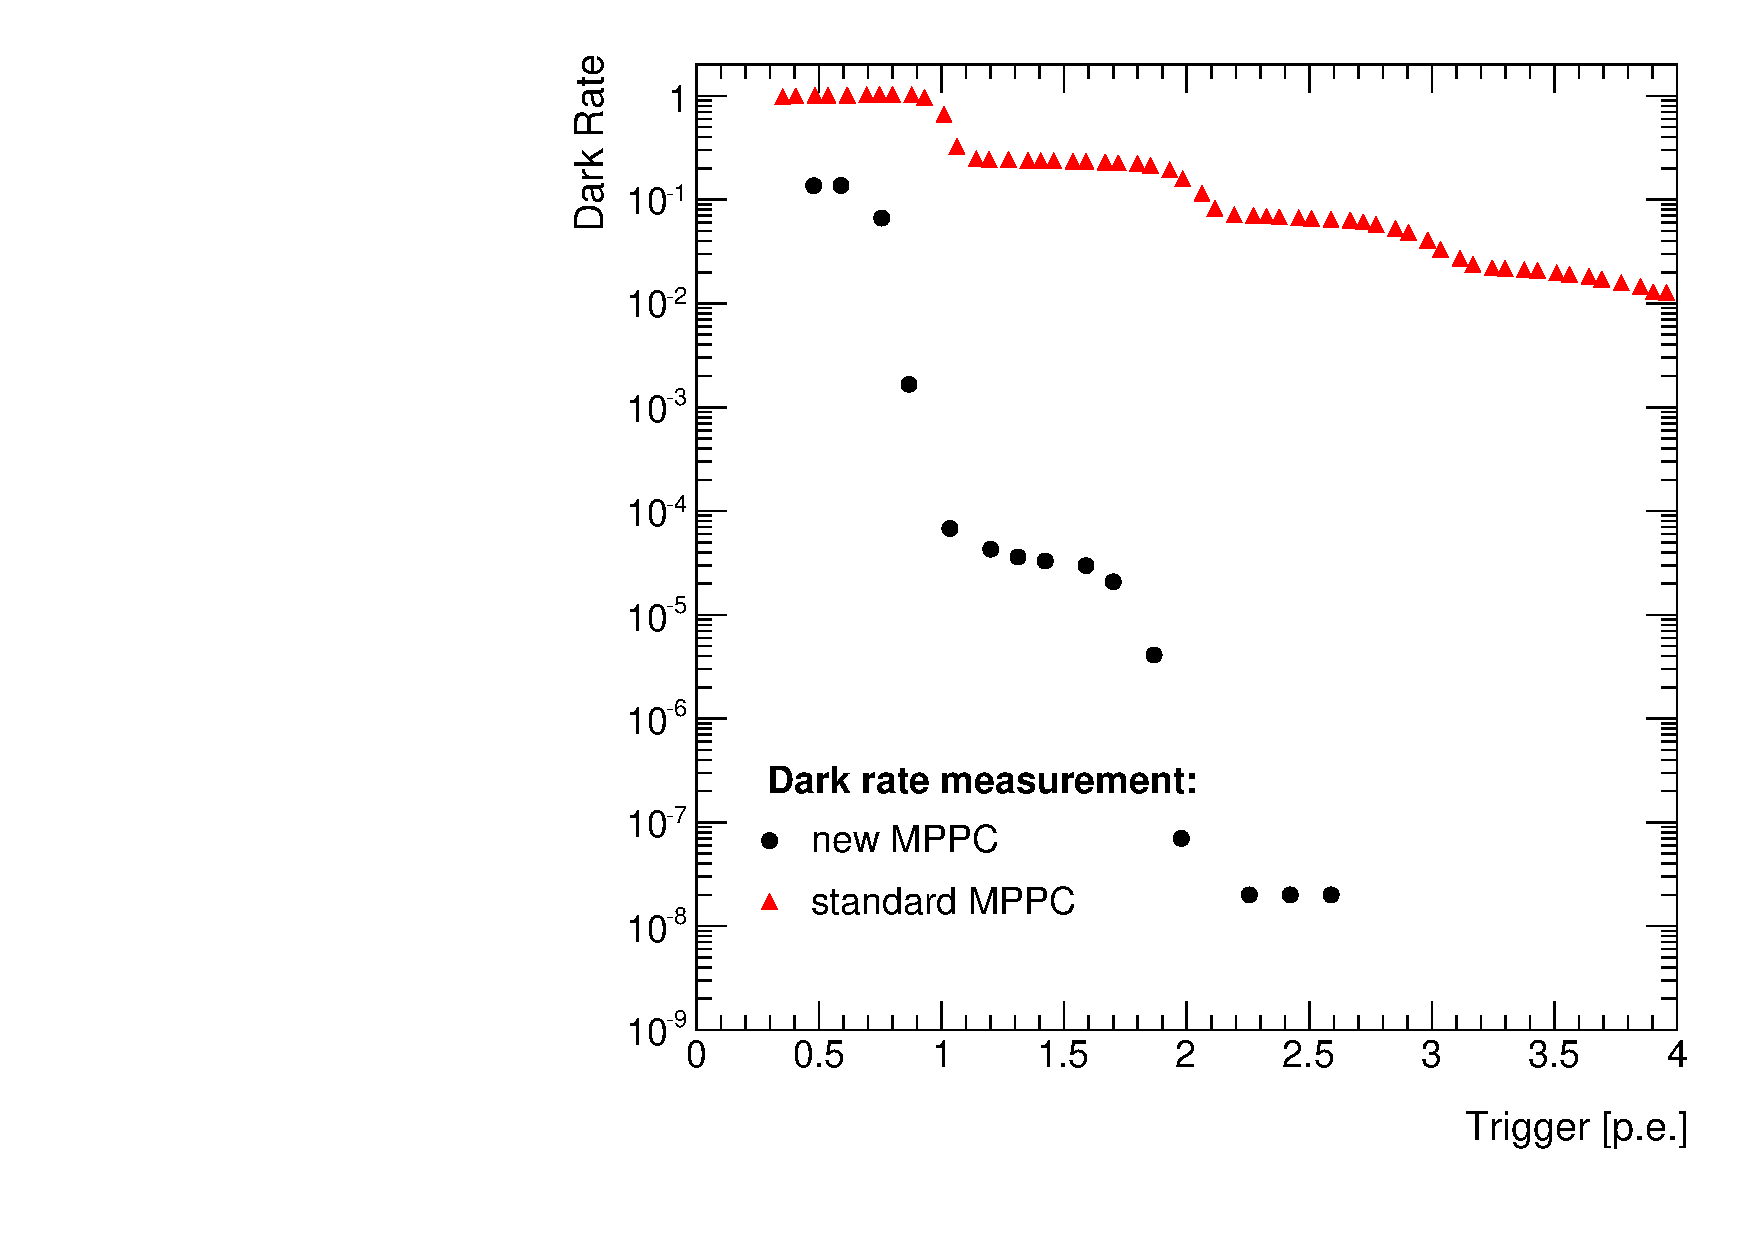
\includegraphics[width=.5\linewidth]{Calorimeter/AHCAL/DarkCount}
	\caption{Dark count rate of recent SiPMs, MPPC devices by Hamamatsu, without (standard) and with (new) inter-pixel cross talk suppression. ({\it Courtesy MPI for Physics, Munich})}
	\label{fig:Calorimeter:AHCAL:DarkCount}
\end{figure}

As a consequence of the wide success of SiPM applications in other fields, e.g. in medical imaging, the development of improved sensors is dynamically pursued in industry, and several groups are in close contact with leading producers. Progress has been made in terms of dark rate (see Figure~\ref{fig:Calorimeter:AHCAL:DarkCount}), noise above MIP threshold and dynamic range. For comparison, typical SiPMs in the first generation prototype had a dark rate of about 2 MHz and a cross talk probability of about 25\%. In addition, the samples are much more homogeneous than at the time of the first prototype, which results in a strong simplification of commissioning and calibration procedures.

In the time since the TDR, scintillator tile SiPM units without wave-length shifting fiber have been developed, based on machined and on injection-moulded tiles, individually wrapped in reflector foil. They have been integrated into a partially instrumented absorber stack and tested with beams at DESY and CERN in 2014 -- 2015.

Industrialization of the SiPM and tile design has been addressed, and assembly procedures with industrial facilities such as automatic pick-and-place machines have been established. 

\begin{figure}
	\centering
	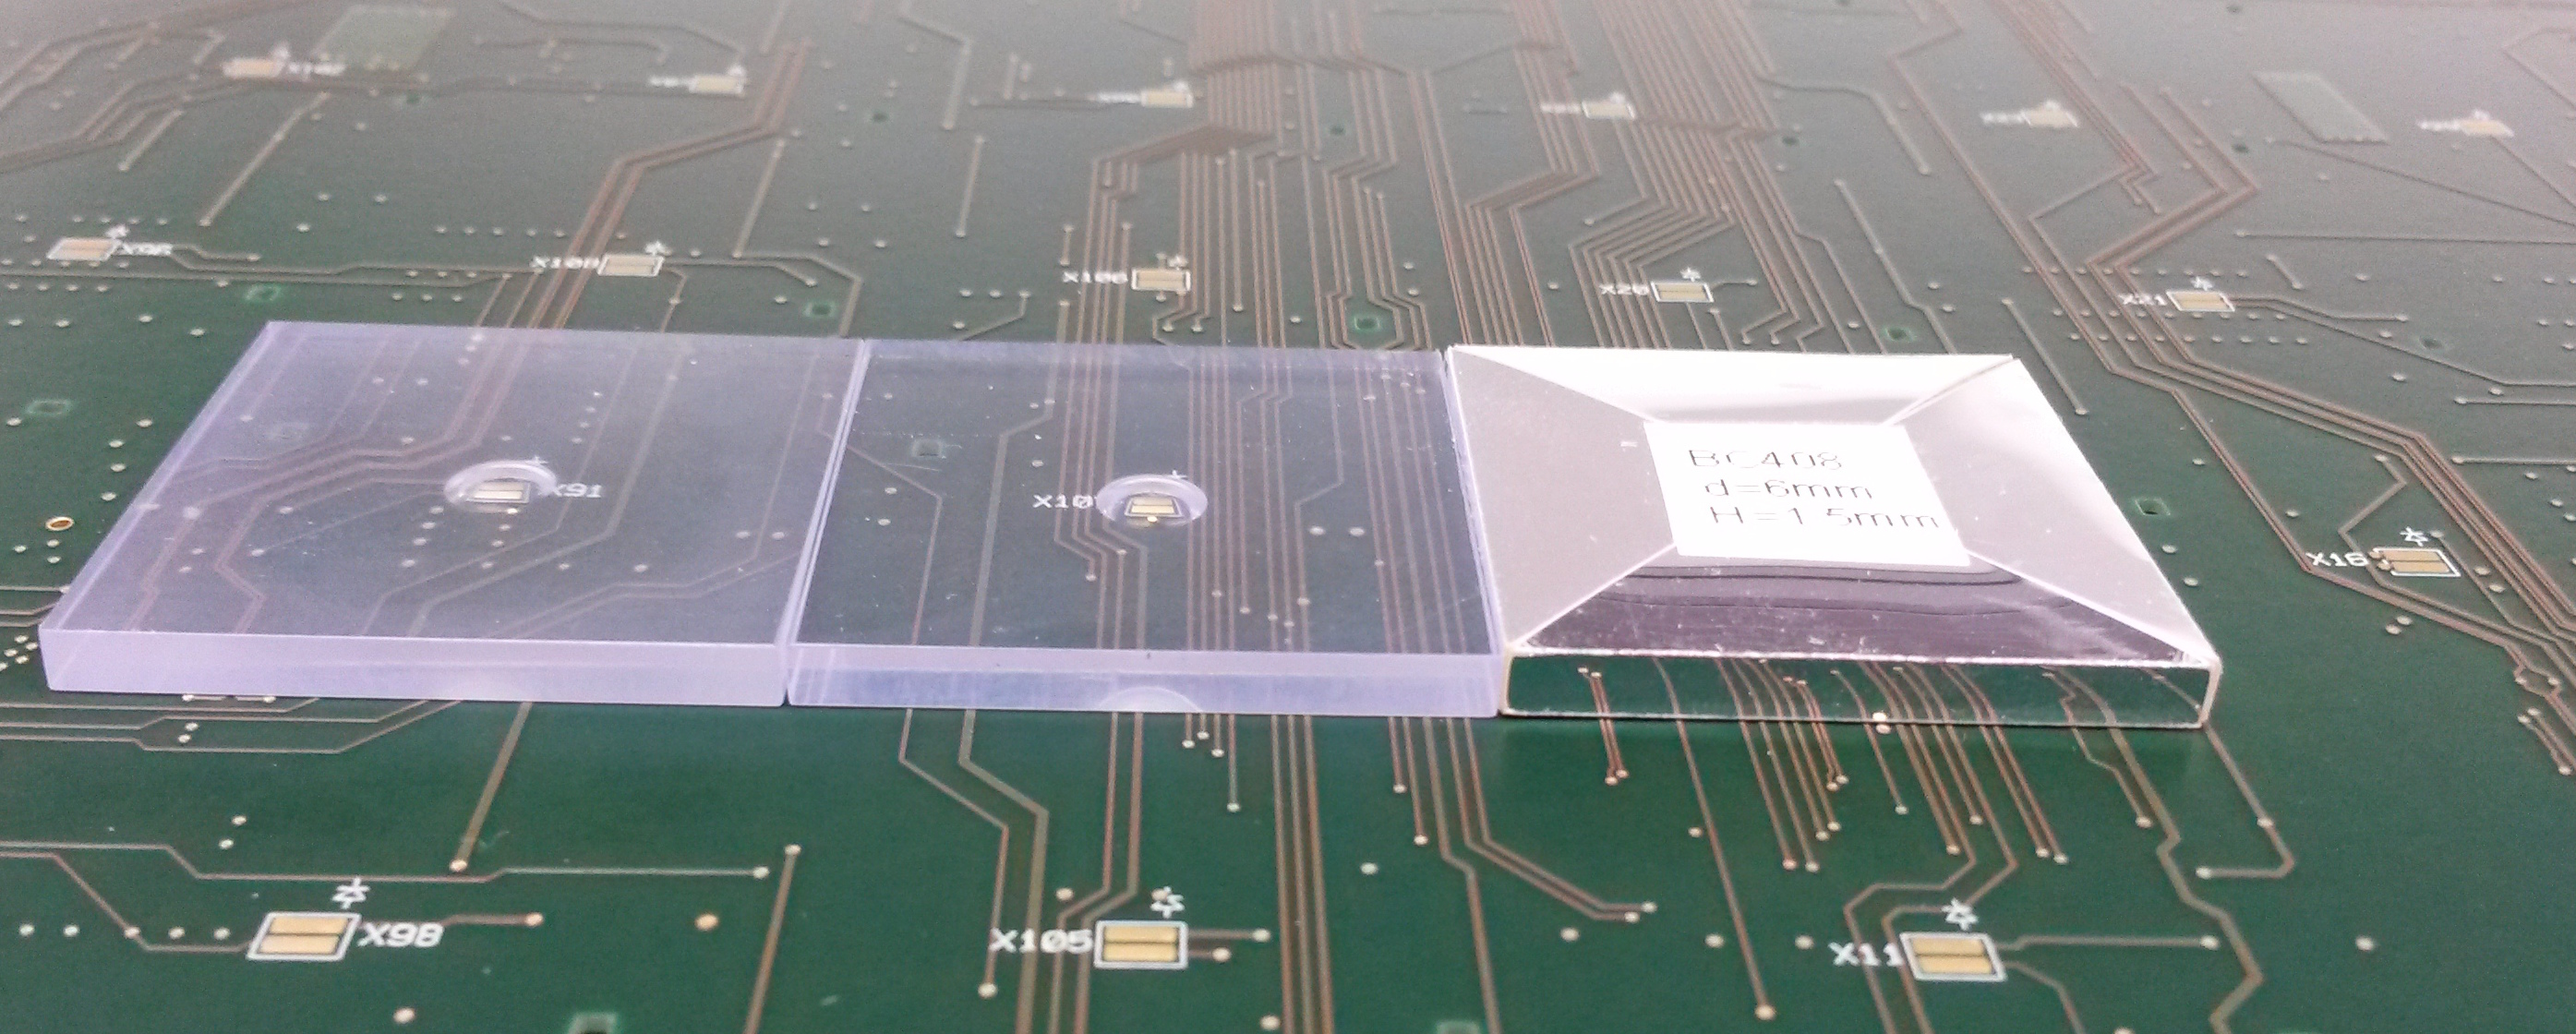
\includegraphics[width=0.5\textwidth]{Calorimeter/AHCAL/SurfaceMountedTiles}
	\caption{AHCAL read-out board with surface-mounted SiPMs and tiles. ({\it Courtesy University of Mainz})}
	\label{fig:Calorimeter:AHCAL:HBU}
\end{figure}

The studies converged on the current design, with photo-sensors integrated in the read-out electronics board, which results in further simplifications, i.e., cost and time savings, but poses higher performance requirements to the SiPM, which can met with the latest generation of SiPMs. This design is shown in Figure~\ref{fig:Calorimeter:AHCAL:HBU}. A quality assurance and integration chain has been worked out that is also scalable to the mass production as required for a LC detector.

\subsubsection{Electronics and active layer integration}

The design of the active layers with integrated read-out ASICs and calibration system had been basically validated in beam tests of a single HCAL layer consisting of four base units (HBUs) at CERN in 2012 and reported in the TDR. An HBU reads $12 \times 12$ tiles with 4 ASICs. The present ASIC belongs to the 2nd generation ROC family used also in ECAL and SDHCAL. An HCAL layer carries interfaces for DAQ, calibration and power supply, which already have a compact design fulfilling space constraints at an ILC detector.

The main functional difference between the integrated electronics and that of the physics prototype is the self-triggered operation and on-detector zero-suppression, which implies much higher demands on controlling the noise behavior and ensuring a stable detector response. It is thus mandatory to re-establish the calorimeter performance with a full-scale beam test, including the operation with fast power cycling. However, this is out of reach with present funding levels.

Further R\&D in the next years has to be done on the ASIC. The 3rd generation ASIC will have a more robust slow control architecture and possibly channel-wise buffer management, which improves rate capabilities. In parallel, an alternative design of the analog part, which can handle a larger range of sensor, has been finished and needs to be integrated into the read-out board and digital data handling.

\subsubsection{Readout System Integration}

\begin{figure}
	\centering
	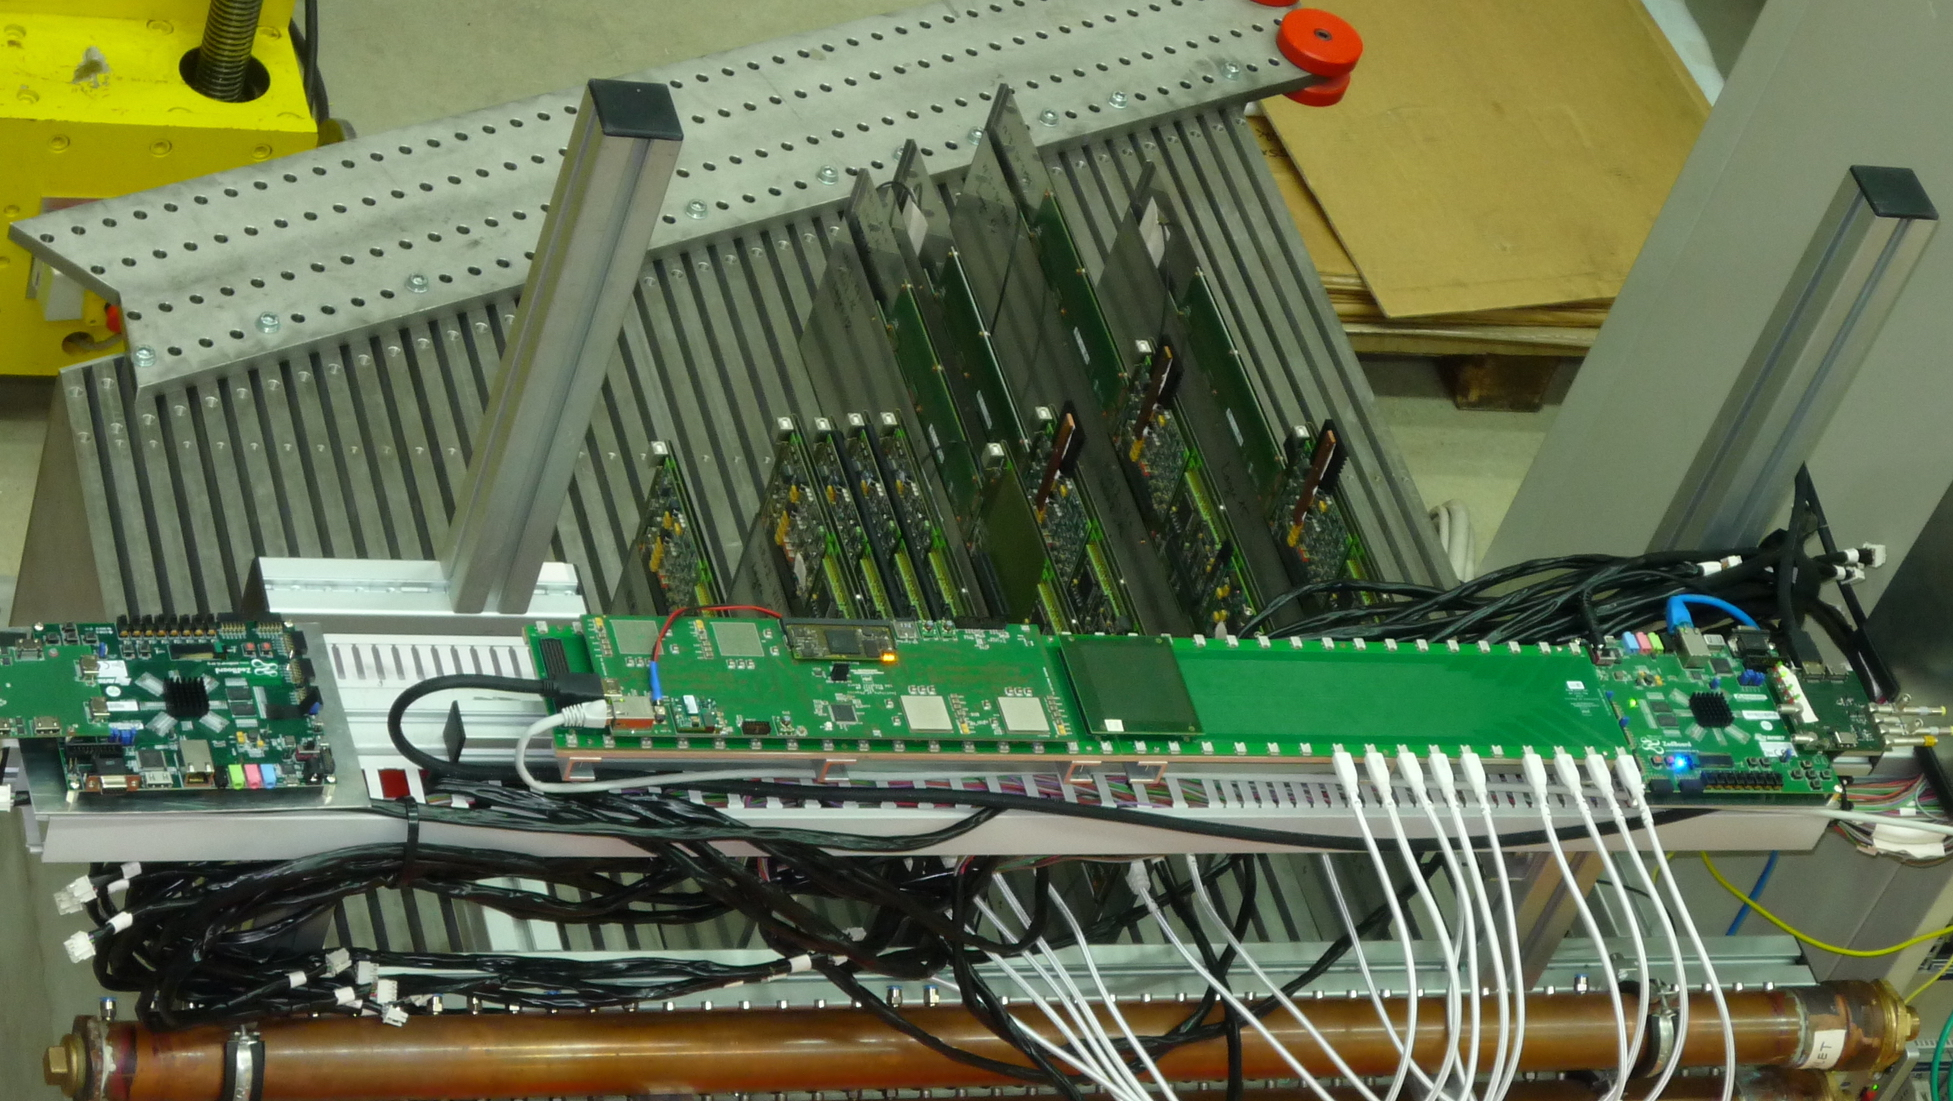
\includegraphics[width=.5\textwidth]{Calorimeter/AHCAL/AHCAL_Stack}
	\caption{Partially instrumented AHCAL stack with integrated read-out electronics and data concentrator for two complete modules.({\it Courtesy DESY})}
	\label{fig:Calorimeter:AHCAL:Stack}
\end{figure}

In parallel to the integration of layers, that of entire stacks or modules has been pursued. Since the TDR release, efforts concentrated on developing a multi-layer DAQ capable of reading larger systems. This was ready for beam tests at CERN in fall 2014. It involves integration of a dedicated module data concentrator (see Figure~\ref{fig:Calorimeter:AHCAL:Stack}), which collects signals from all layers of two phi-sectors for sending them to the off-detector data receiver. The HCAL DAQ has been integrated into the higher level system EUDAQ2 for the purpose of combined beam tests, for example with a tracking device for uniformity studies, or with an ECAL for inter-calibration and combined performance. The same is true for slow control data.

A power supply system based on commercially available modules has been set up; an alternative custom system with optimized channel density per module is being developed.

It has been demonstrated that temperature-induced variations of the SiPM gain can be compensated by adjusting the bias voltage. The approach stabilizes the detector response and trigger efficiency and thus simplifies operations significantly. Automatic procedures based on this principle have been developed and implemented at system level.

\subsubsection{Infrastructure for production, quality assurance and characterisation}

The AHCAL is probably the sub-detector with the largest number of individual components. While the number of electronics boards, layers and interfaces is similar to other ECAL or HCAL options, the large quantity of tiles and SiPMs deserves special attention. This affects production and also quality assurance.

While it would be premature to build up full production infrastructure, already for the second generation full-scale prototype with its 22000 channels, conceptual solutions had to be developed and exercised using demonstrators, which could be seen as prototypes of future installations.

Spot-samples of all 40 SiPM lots, and each one of the 640 ASICs, had undergone semi-automatic testing procedures before soldering the HBUs. Without any further surface treatment, injection-moulded scintillator tiles have been wrapped in laser-cut reflective foil by a robotic procedure and mounted on the HBUs using a pick-and-place machine, after glue dispensing with a screen printer. Cosmic test stands were used to assure the quality of the assembly, to monitor the uniformity of the light yield over the production period and within HBUs, and to obtain an initial MIP calibration.

\subsubsection{Prototype integration and test beam operation}
 The HBUs have been integrated into cassettes with interfaces for DAQ, LED pulsing and power distribution, which provide active compensation of temperature variations by automatic adjustments of the common bias voltage of the photon sensors in each layer. Figure~\ref{fig:AHCAL:ActiveLayer} shows the top side of one active layer, with the scintillator tiles visible. All layers have been calibrated in the DESY test beam, and all channels except eight (0.4‰) are working.

 \begin{figure}
	\centering
	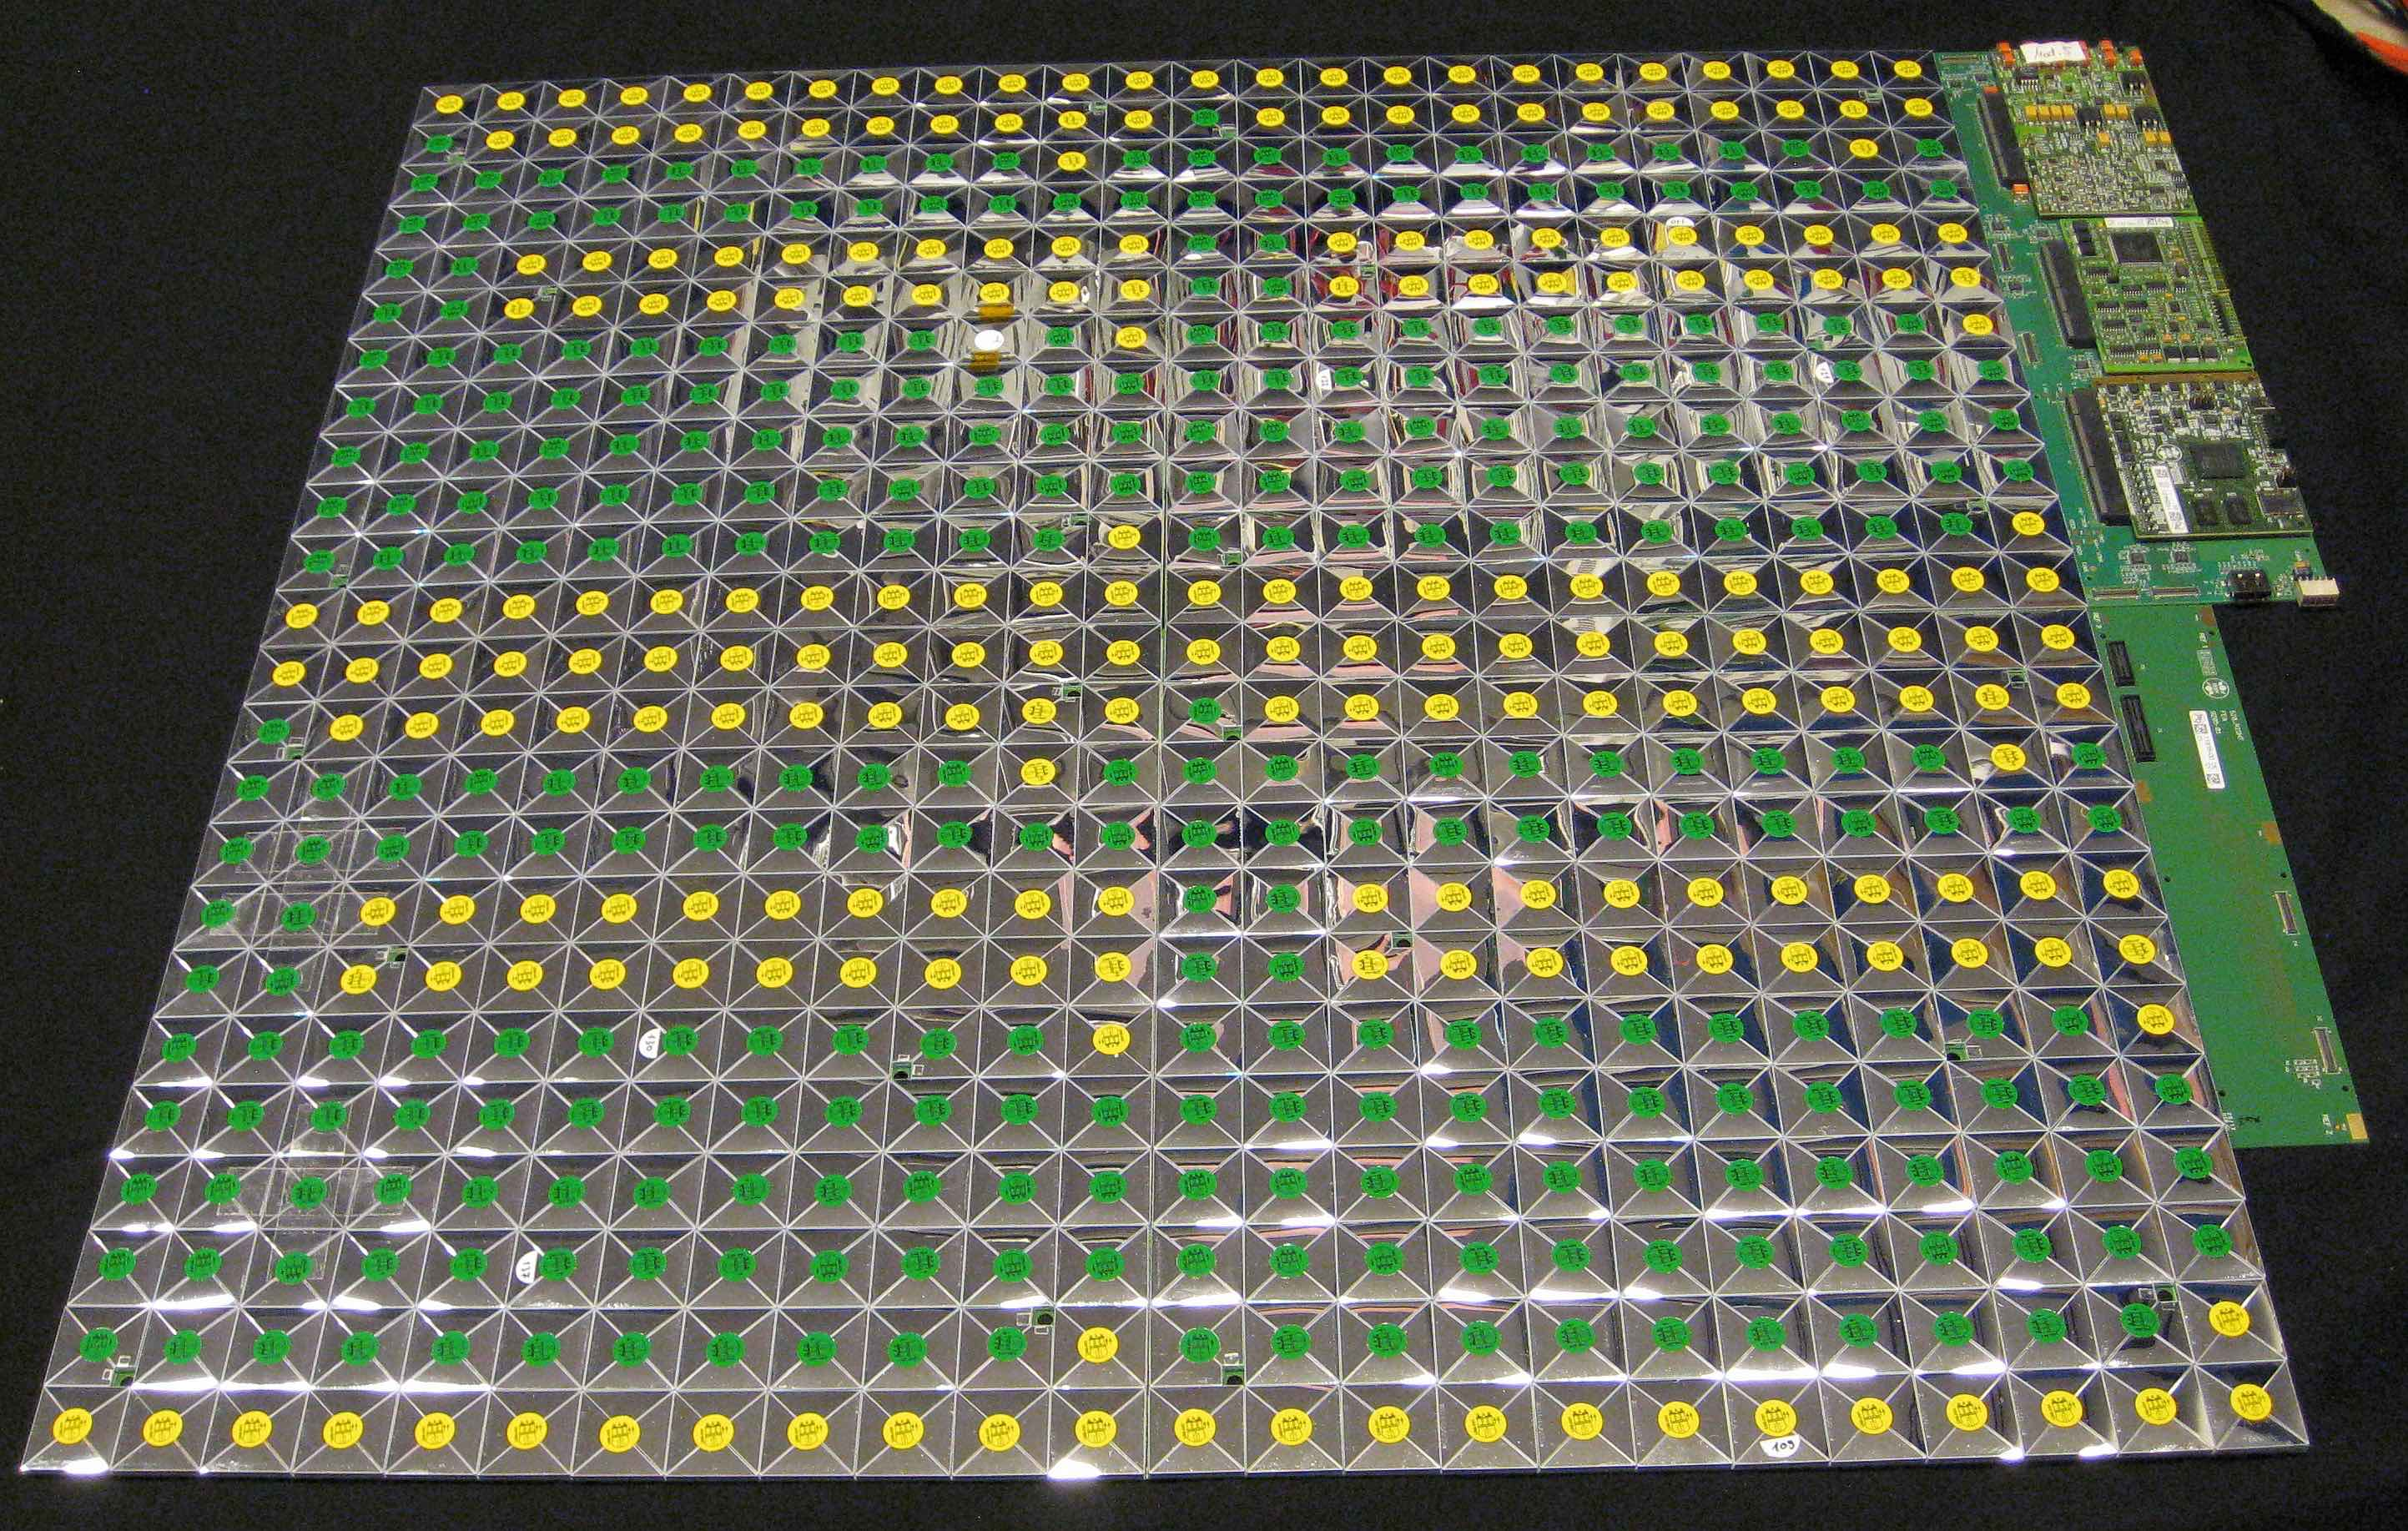
\includegraphics[width=.5\linewidth]{Calorimeter/AHCAL/AHCalActiveLayer}
	\caption{AHCAL active layer side with wrapped tiles on 4 HBUs, with interfaces for DAQ, LEDs and power. ({\it Courtesy DESY})}
	\label{fig:AHCAL:ActiveLayer}
 \end{figure}

Finally, the calibrated layers were assembled into the absorber stack and connected to data concentration, power distribution and cooling services. Figure~\ref{fig:AHCAL:FullStack} shows the active layers with connected services inserted in the absorber structure. The full prototype has been commissioned with cosmic muons, exploiting its self-triggering capabilities.

\begin{figure}
	\centering
	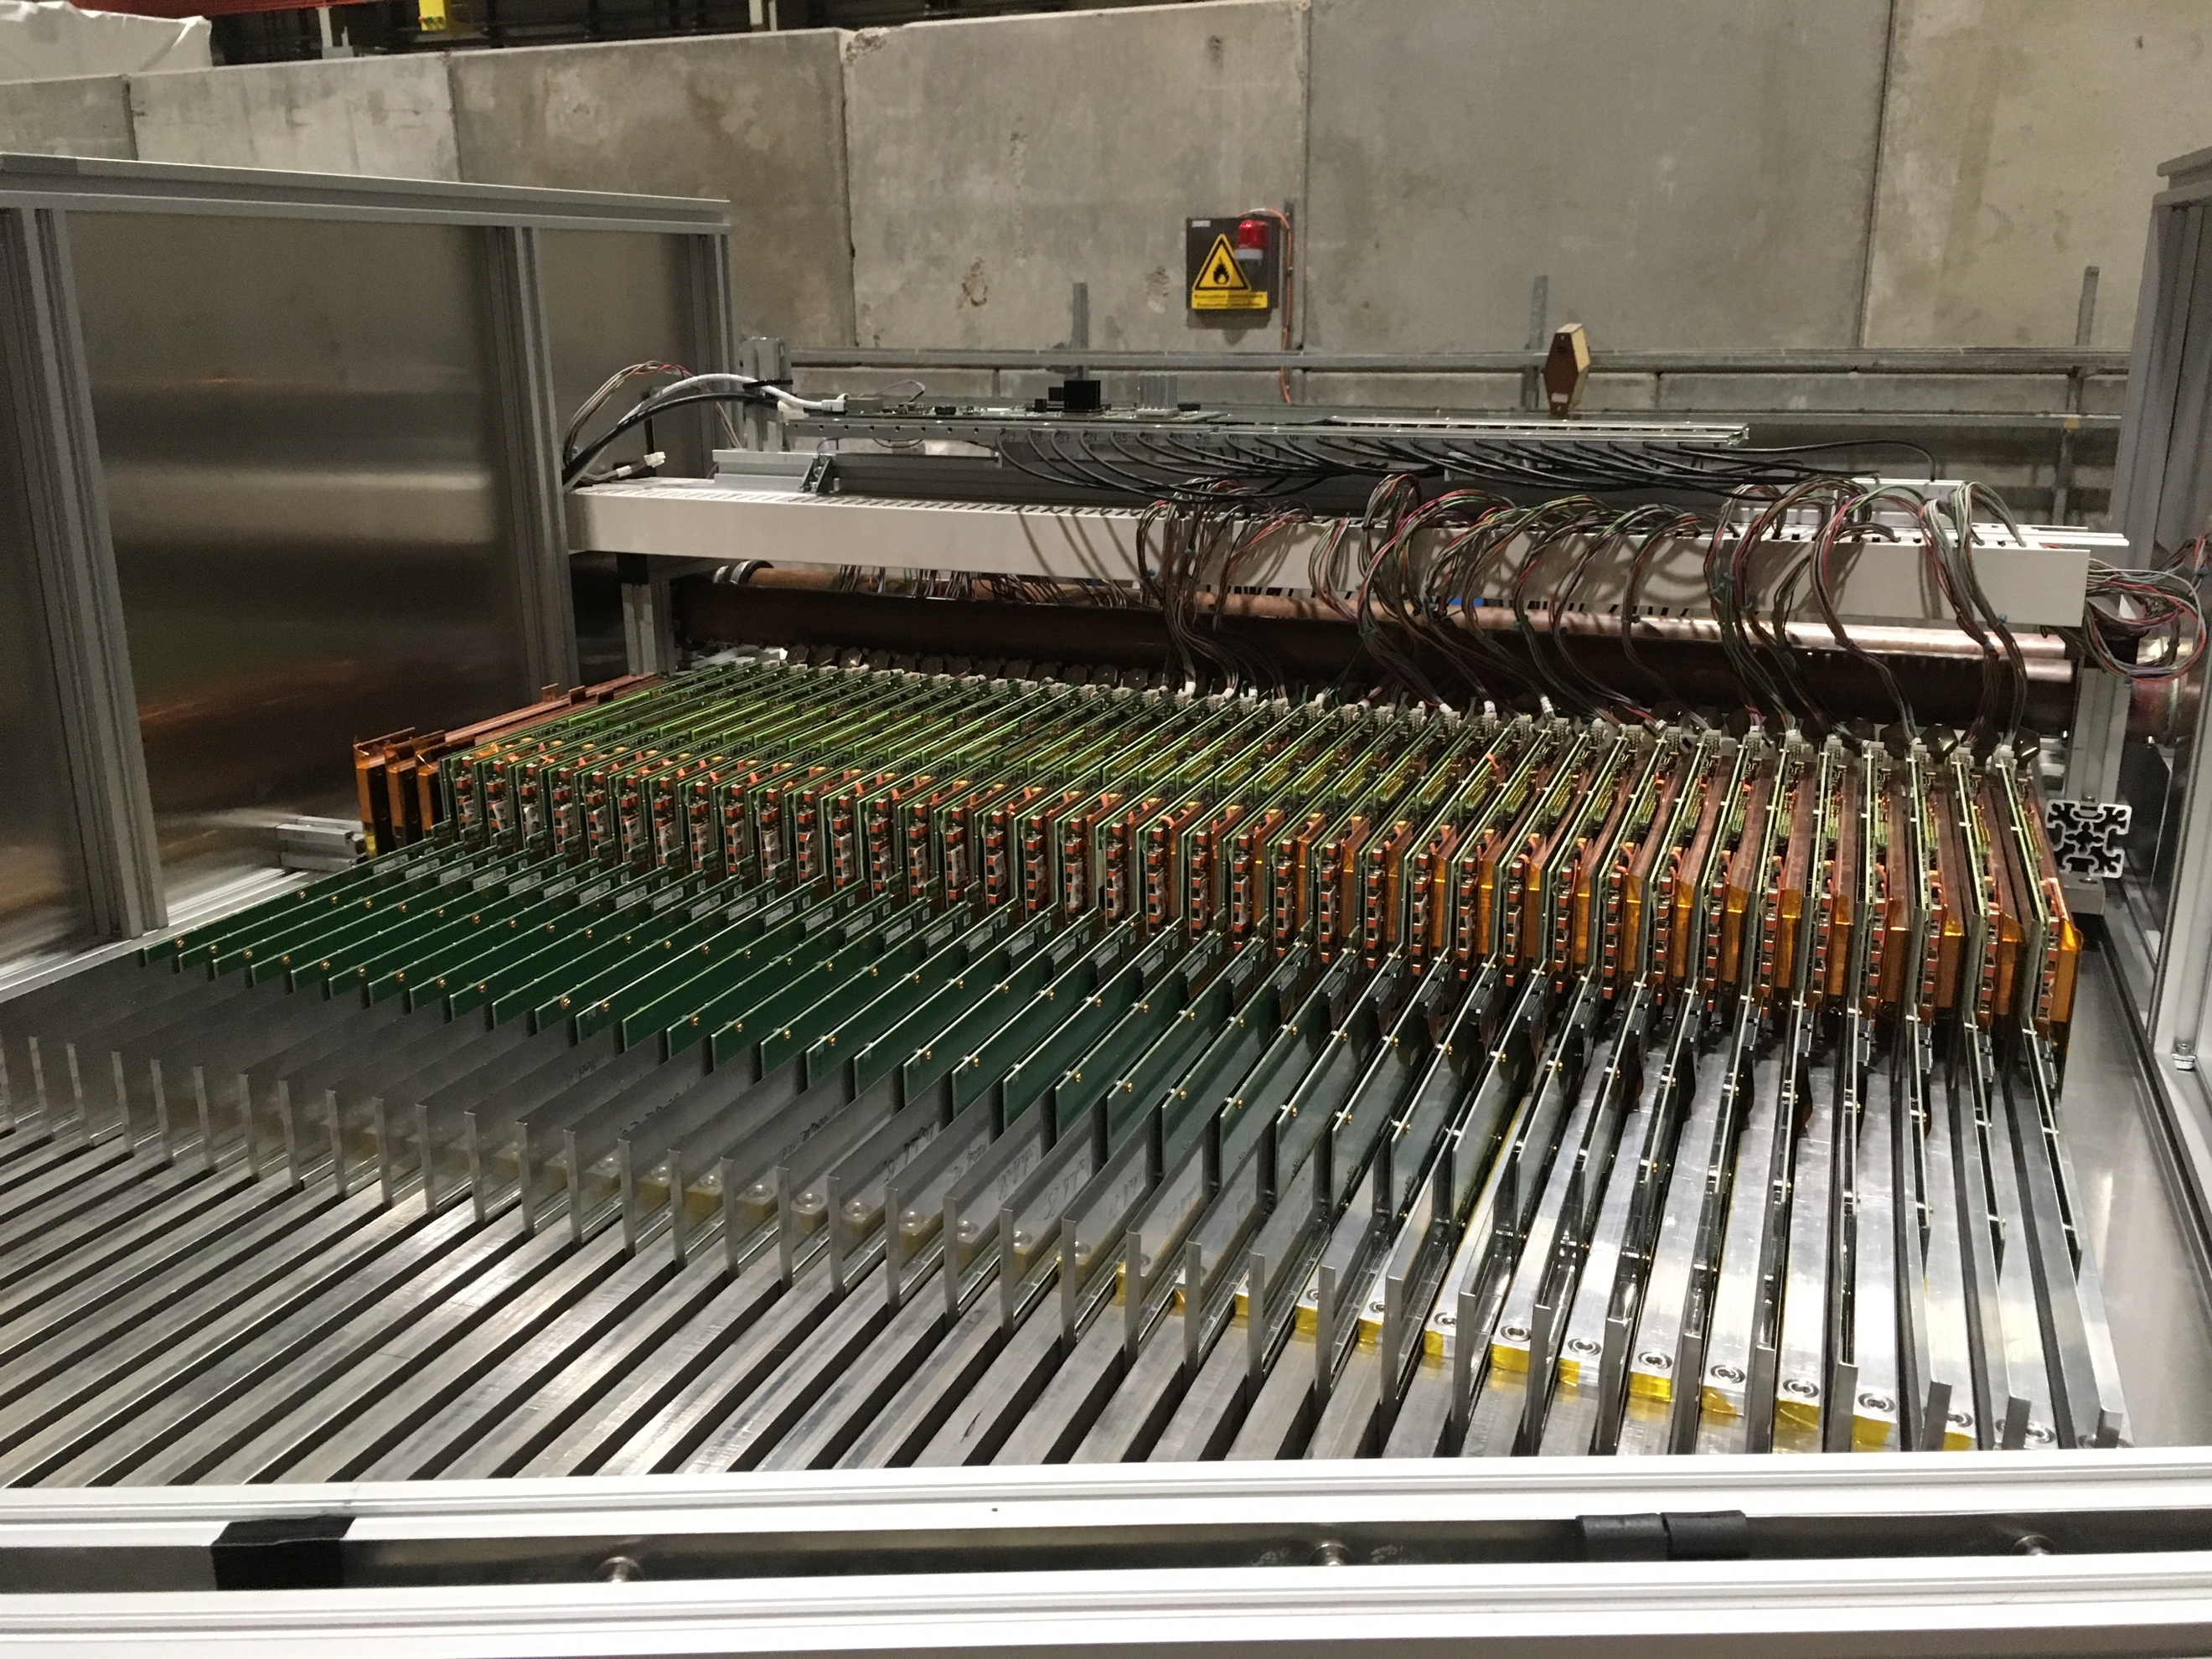
\includegraphics[width=.5\linewidth]{Calorimeter/AHCAL/AHCalStack}
	\caption{Fully integrated SiPM-on-tile AHCAL engineering prototype. ({\it Courtesy DESY})}
	\label{fig:AHCAL:FullStack}
\end{figure}

The prototype has been installed in the test beam for data taking at the CERN SPS. In two periods in May and in June 2018, several $10^7$ events with muon tracks as well as electron and pion showers at various energies in the range from 10 GeV up to 100 GeV for electrons and 200 GeV for hadrons have been collected. The data taking rate averaged over the about 5s long spills and was up to 400 events per second. Figure~\ref{fig:AHCAL:EvtDisplay} shows two event displays, a cosmic muon and a high-energy pion shower.

\begin{figure}
	\centering
	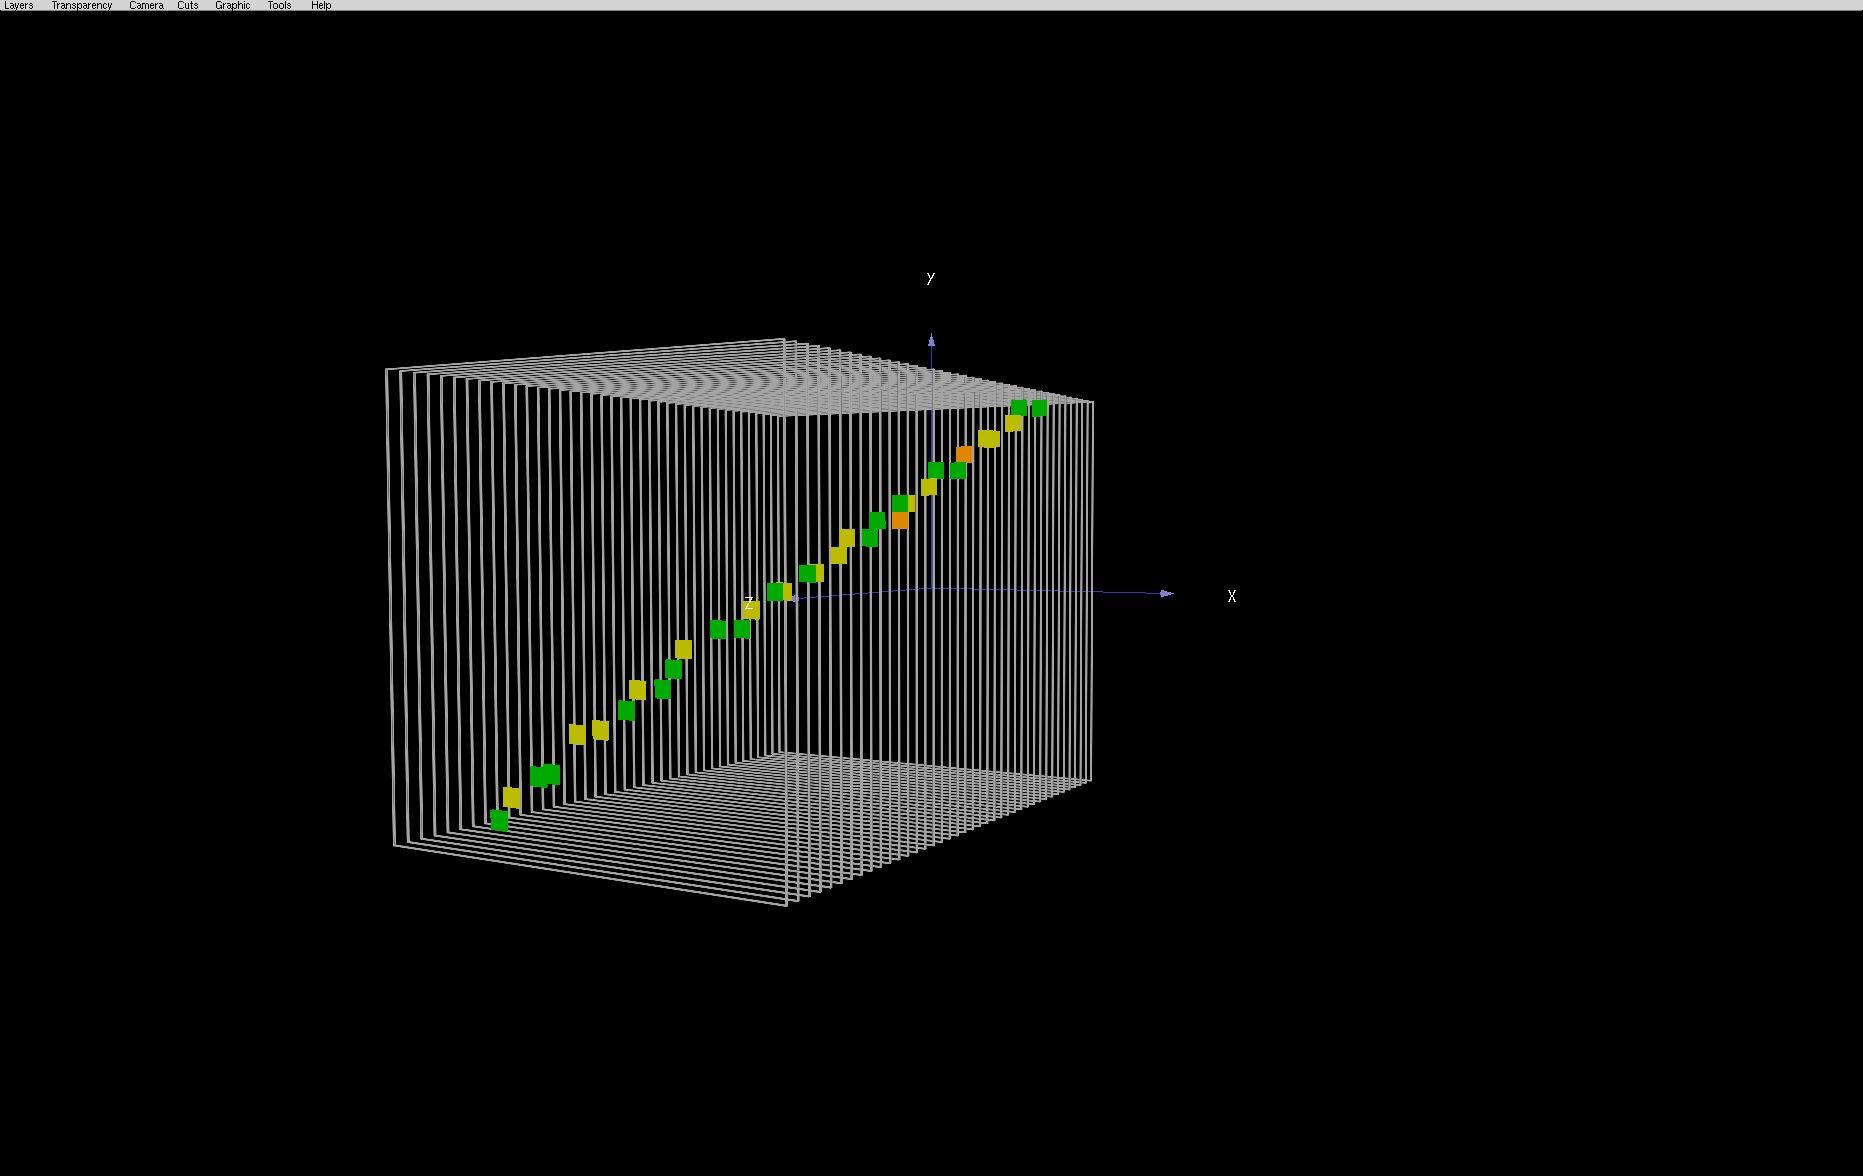
\includegraphics[width=.49\linewidth]{Calorimeter/AHCAL/AHCalEvtDisplay1}
	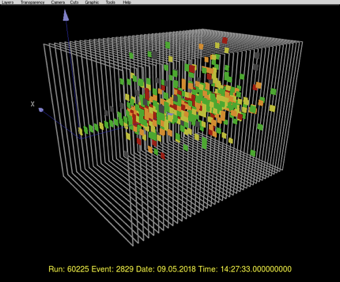
\includegraphics[width=.49\linewidth]{Calorimeter/AHCAL/AHCalEvtDisplay2}
	\caption{AHCAL event displays: cosmic muon and high energy pion ({\it Courtesy DESY})}
	\label{fig:AHCAL:EvtDisplay}
\end{figure}

The rich data sample collected in the two test beam periods in 2018 will be used for shower separation studies based on 5-dimensional reconstruction algorithms exploiting the high spatial, energy and time resolution of this novel detector.

\subsubsection{Mechanics and Cooling}

The absorber structure bears more challenges than for conventional hadronic calorimeters. Due to the much finer longitudinal segmentation and the imperative to minimize the total radius inside the coil, there are many active gaps with tight tolerances. A design has been developed and prototyped, which achieves the required tolerances with a cost-effective roller-leveling process without machining off excess material. Two test structures have been built; one -- used also for the test beam prototype -- covers the full transverse cross section of a barrel module, the other the full lateral extension. The cassettes housing the active elements have the final design and are used in beam tests.

These structures need to be investigated with respect to their robustness against earthquakes. Simulations of the whole ILD structure have been made, and measurements on the test structures exposed to accelerating forces should be done in order to check the simulations. The results of the simulation will be used to optimize the structural design.

A cooling system has been developed. The ASICs integrated in the detector layers are power-pulsed and do not need active cooling, but the interfaces, in particular the power regulators, do. The solution developed for beam tests is already laid out for a leak-less under-pressure based system.

As enough active elements become available for instrumenting several active layers at full size, the thermal simulations should be verified with measurements using the second lateral test structure, too. This will constitute an important step in system integration, as it addresses the issues associated with large layers and in particular power distribution, power cycling and heat dissipation.

\subsection{Summary}
The AHCAL effort has produced a number of significant results in the time since the ILC TDR:
\begin{itemize}
\item Publication of 7 journal papers and 4 preliminary conference results in the form of internally reviewed notes, on Geant 4 validation with pions and protons in steel and tungsten, including new observables like track segments
\item Development, construction and beam test of a second-generation full-size prototype with a new, simplified tile SiPM system with improved sensor performance, using a design and production and QA procedures scalable to a full ILC detector
\end{itemize}

\subsection{Future Plans}

The AHCAL has accomplished the essential step towards a technical design report with a realistic full-scale prototype. Coordinated R\&D is required in the following areas:

\begin{itemize}
\item 2nd generation prototype reconstruction and simulation software
\item Development of timing reconstruction
\item Analysis of 2nd generation test beam data
\end{itemize}

\subsection{Engineering Challenges}

Electronics:
\begin{itemize}
\item establish power-pulsed operation of large layers
\item 3rd generation ASIC of ROC family
\item ASIC for larger range of SiPM gains
\end{itemize}

Absorber structure:
\begin{itemize}
\item Earthquake stability calculations and tests
\item Thermal tests with full-scale instrumented and powered structures
\end{itemize}

There are ample opportunities for new groups to join into any of these fields, depending on the special competences they wish to contribute.
